\section{Lagrangian Finite Element Methods}

\label{sec:lagrange}

In this work, we are looking at Lagrangian FEM on structured rectilinear grids,
also known as Tensor-Product Lagrangian FEM \cite{hiptmair_numerical_2023}.

The Lagrangian finite element space defines a set of piecewise continuous
polynomials of degree $p$ over the mesh. They are only piecewise over the element boundaries.

\begin{definition}[(Tensor-product) Lagrangian finite element spaces]
    We define the space of $p$-th degree
    Lagrangian finite element functions on a tensor product mesh $\mathcal{M}$ as \cite{hiptmair_numerical_2023}:
    \begin{align}
        \mathcal{S}_p^0(\mathcal{M}) := \{ v \in C^0(\bar{\Omega}):
        v_{|K} \in \mathcal{Q}_p(K) \ \forall K \in \mathcal{M}\},
    \end{align}
    where $\bar{\Omega}$ is the domain of the mesh, including the boundary,
    $\mathcal{Q}_p(K)$ is the set of basis functions that are tensor products of polynomials of degree $p$ spanning the element $K$
    and $v_{|K}$ are the functions $v$ restricted to element $K$.

    The space $\mathcal{S}_p^0$ contains continuous, piecewise polynomial functions
    that are made up of ``stitched together'' basis functions functions from the elementes in mesh $\mathcal{M}$.
\end{definition}

\subsection{Lagrangian shape functions}

Together with the Lagrangian finite element space, the basis functions have to be defined as well.
The basis functions are defined according to the policy of interpolation nodes through the cardinal
basis property (see def. \ref{def:cardinal_basis_property}).

\begin{definition}[Lagrange Polynomials]
    Given a set $\{ x_0, ..., x_n\} \subset \R$ of nodes, the \emph{Lagrange polynomials} are \cite{hiptmair_numerical_2020}
    \begin{align}
        L_i(x) := \prod_{j=0, j\neq i}^n \frac{x - x_i}{x_i - x_j}, \quad i=0, ..., n.
    \end{align}
\end{definition}

The Lagrange interpolating polynomial is the unique
polynomial of the lowest degree that interpolates a set of points \cite{hiptmair_numerical_2020}.
They satisfy the cardinal basis property on the interpolation nodes.

To define polynomial functions of degree $p$ on the elements, Lagrangian FEM utilizes
Lagrangian polynomials, hence the name.
We have a fixed number of degrees of freedom (DOFs) per element that correspond to the
local shape functions of the element.
The shape functions satisfy the cardinal basis property that they evaluate to one
at the location of the corresponding DOF and to zero at the locations of all the other DOFs.

\subsubsection{First-order shape functions}

In one dimension, first-order Lagrangian shape functions are polynomials of degree 1,
or linear polynomials, and interpolate two points.
The basis functions for first-order Lagrangian FEM are the well-known tent functions \cite{hiptmair_numerical_2023}.
The shape functions are:

\begin{align}
    \hat{b}^i(x) = \begin{cases}
                       1 - x & i=0, \\
                       x     & i=1.
                   \end{cases}
\end{align}

See figure \ref{fig:1_lagrange_1d} for a plot of 1D first-order Lagrangian shape functions.

\begin{figure}[h]
    \centering
    \begin{tikzpicture}
        \begin{axis}[domain=0:1,samples=100]
            \addplot[no markers, color=red, thick] {1 - x};
            \addplot[no markers, color=blue, thick] {x};
            \addplot[name path=xaxis, black] {0};

            \node[circle, fill=red, inner sep=2pt] at (axis cs:0,0) {};
            \node[circle, fill=red, inner sep=2pt] at (axis cs:0,1) {};

            \node[circle, fill=blue, inner sep=2pt] at (axis cs:1,0) {};
            \node[circle, fill=blue, inner sep=2pt] at (axis cs:1,1) {};

        \end{axis}
    \end{tikzpicture}
    \caption{First-order Lagrange shape functions.}
    \label{fig:1_lagrange_1d}
\end{figure}

In two dimensions, the first-order Lagrangian shape functions are the tensor-product
of 1D 1st-order shape functions of the y- and the x-dimension:

\begin{align}
    \hat{b}^i(x, y) = \begin{cases}
                          (1-x)(1-y) & i=0, \\
                          x(1-y)     & i=1, \\
                          xy         & i=2, \\
                          (x-1)y     & i=3.
                      \end{cases}
\end{align}

See figure \ref{fig:lagrange_1st_2d} for a plot of 2D first-order Lagrangian shape functions.

\begin{figure}[h]
    \centering
    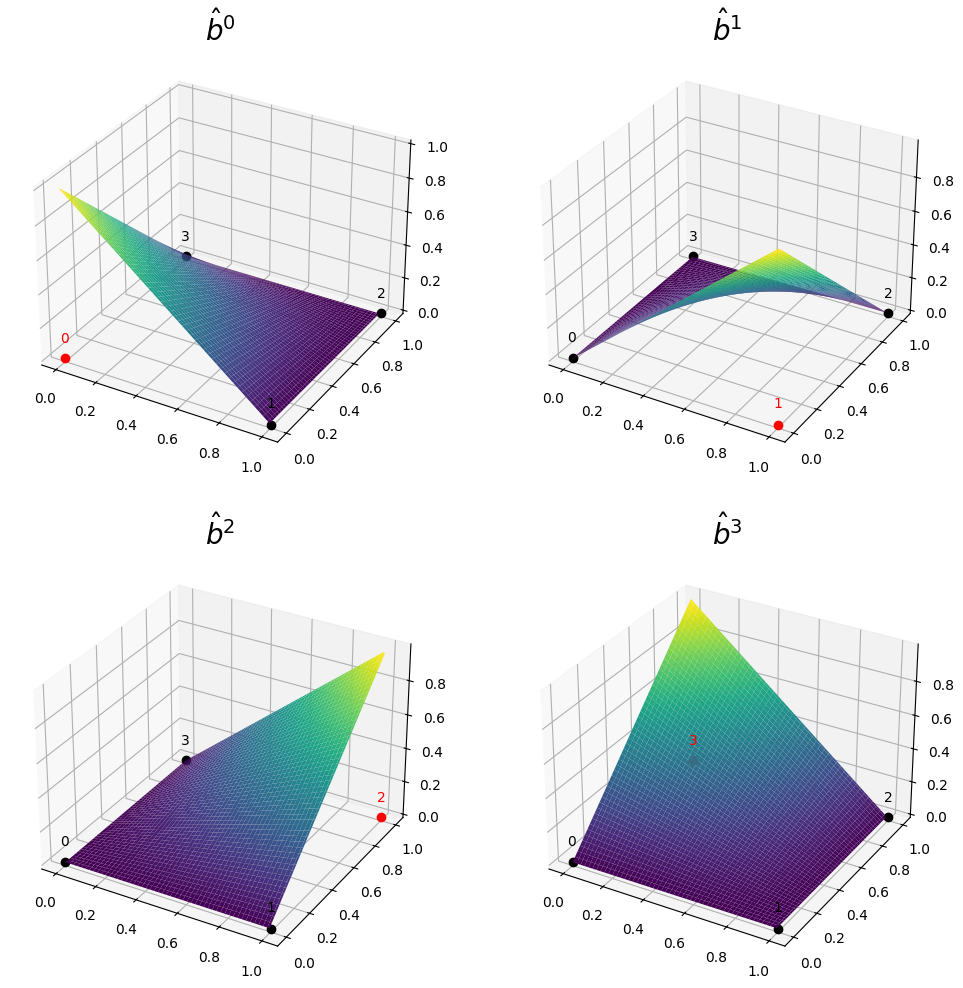
\includegraphics[width=\hsize-2cm]{pictures/lagrange_1st_basis_2d.png}
    \caption{First-order Lagrangian shape functions in 2D.}
    \label{fig:lagrange_1st_2d}
\end{figure}

\subsubsection{Higher-order shape functions}

Higher-order Lagrangian methods have more degrees of freedom per element.
Second-order Lagrangian finite element methods have an additional degree of freedom
in the middle of each edge, in two dimensions also a degree of freedom in the middle of each face
and in three dimensions also an additional degree of freedom in the middle of each cell.

In 1D the shape functions are polynomials of degree two,
specifically, the Lagrangian interpolation polynomials interpolating the points
$0$, $\frac{1}{2}$ and $1$:

\begin{align}
    \label{eq:lagrange_1d_2nd}
    \hat{b}^i(x) = \begin{cases}
                       (1-x)(\frac{1}{2} - x) & i=0, \\
                       x(1-x)                 & i=1, \\
                       x(\frac{1}{2} - x)     & i=2.
                   \end{cases}
\end{align}

\begin{figure}[h]
    \centering
    \begin{tikzpicture}
        \begin{axis}[domain=0:1,samples=100]
            \addplot[name path=b0, no markers, color=red, thick] {2 * (x - 0.5) * (x - 1)};
            \addplot[name path=b1, no markers, color=blue, thick] {-4 * x * (x - 1)};
            \addplot[name path=b2, no markers, color=DarkMagenta, thick] {2 * x * (x - 0.5)};
            \addplot[name path=xaxis, black] {0};

            \node[circle, fill=red, inner sep=2pt] at (axis cs:0,0) {};
            \node[circle, fill=red, inner sep=2pt] at (axis cs:0,1) {};

            \node[circle, fill=blue, inner sep=2pt] at (axis cs:0.5,0) {};
            \node[circle, fill=blue, inner sep=2pt] at (axis cs:0.5,1) {};

            \node[circle, fill=DarkMagenta, inner sep=2pt] at (axis cs:1,0) {};
            \node[circle, fill=DarkMagenta, inner sep=2pt] at (axis cs:1,1) {};
        \end{axis}

    \end{tikzpicture}
    \caption{Second-order Lagrange shape functions.}
    \label{fig:2_lagrange_1d}
\end{figure}

The definition for even higher-order Lagrangian finite element spaces and shape functions
follows from the definition of the second-order Lagrangian shape functions (Eq. \ref{eq:lagrange_1d_2nd})
and the interpolating polynomials for more degrees of freedom.

\begin{figure}[h]
    \centering
    \begin{tikzpicture}
        \begin{axis}[domain=0:1,samples=100]
            \addplot[name path=b0, no markers, color=red, thick] {-(9*x^3) / 2 + 9*x^2 - ((11 * x) / 2) + 1};
            \addplot[name path=b2, no markers, color=blue, thick] {(9 * x * (3 * x^2 - 5 * x + 2)) / 2};
            \addplot[name path=b1, no markers, color=DarkMagenta, thick] {(9*x * (-3*x^2 + 4*x - 1)) / 2};
            \addplot[name path=b3, no markers, color=DarkGreen, thick] {(x * (9 * x^2 - 9 * x + 2)) / 2};
            \addplot[name path=xaxis, black] {0};

            \node[circle, fill=red, inner sep=2pt] at (axis cs:0,0) {};
            \node[circle, fill=red, inner sep=2pt] at (axis cs:0,1) {};

            \node[circle, fill=blue, inner sep=2pt] at (axis cs:1/3,0) {};
            \node[circle, fill=blue, inner sep=2pt] at (axis cs:1/3,1) {};

            \node[circle, fill=DarkMagenta, inner sep=2pt] at (axis cs:2/3,0) {};
            \node[circle, fill=DarkMagenta, inner sep=2pt] at (axis cs:2/3,1) {};

            \node[circle, fill=DarkGreen, inner sep=2pt] at (axis cs:1,0) {};
            \node[circle, fill=DarkGreen, inner sep=2pt] at (axis cs:1,1) {};

        \end{axis}

    \end{tikzpicture}
    \caption{Third-order Lagrange shape functions.}
    \label{fig:3_lagrange_1d}
\end{figure}


\subsection{LagrangeSpace class}
\label{sec:lagrange_class}

The \texttt{LagrangeSpace} class inherits from the \texttt{FiniteElementSpace} class and
overrides and defines the virtual degree of freedom and assembly member functions.

The \texttt{LagrangeSpace} class does not represent the Lagrangian finite element space in a mathematical sense.
It instead serves as a container for all the DOF and assembly operations
corresponding to the rules implied by the Lagrangian finite element space for a specified order.

It takes template arguments for the floating point type \texttt{T}, the dimension \texttt{Dim},
the order \texttt{Order} as well as an argument for the type of the reference element,
the type of the quadrature rule and left-hand-side and right-hand-side field types.

To inherit from the \texttt{FiniteElementSpace} class, it also has to pass a template argument for the
number of element degrees of freedom \texttt{NumElementDOFs}, which is computed at compile
time from the mesh dimension and the order of the \texttt{LagrangeSpace}.
